\subsection{Performance from finger knuckle images\label{fk-performance}}

\begin{figure}[ht]
    \centering
    \subfloat[]{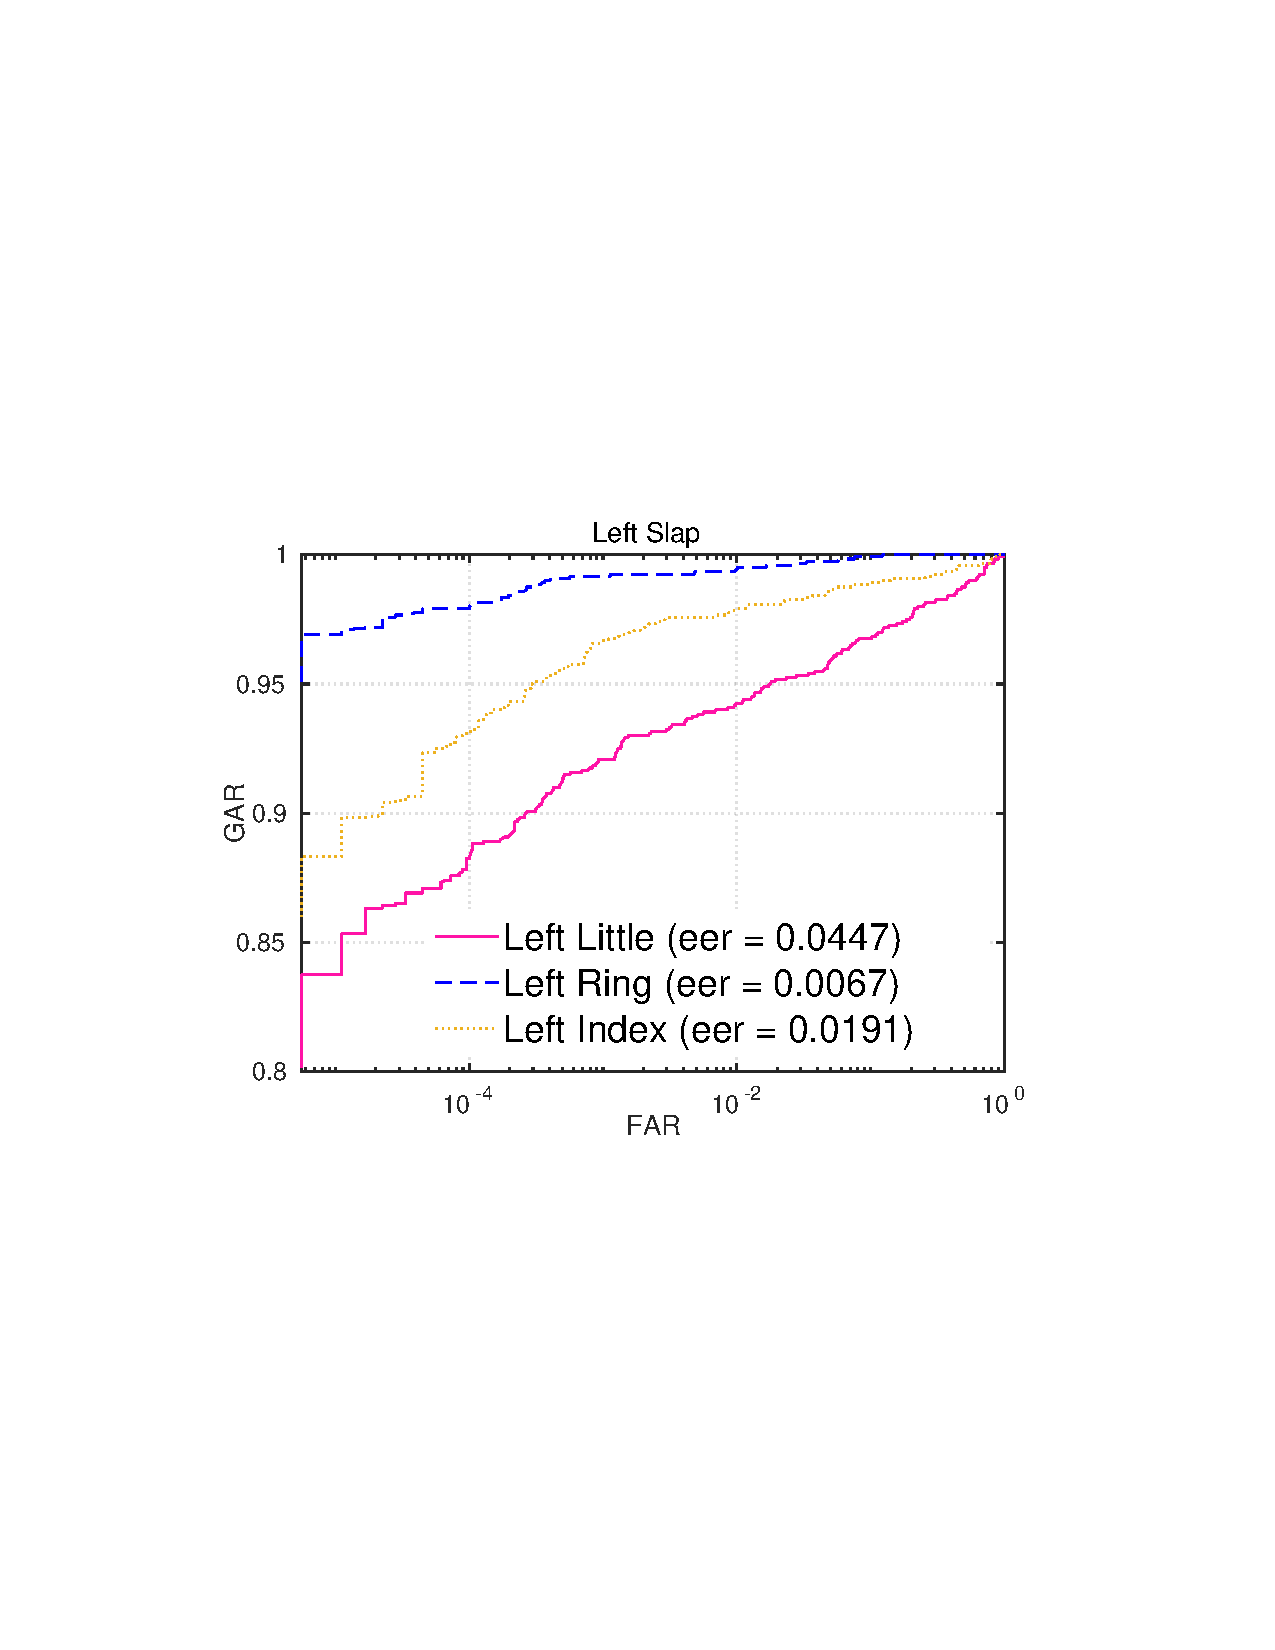
\includegraphics[width=1.7in]{Figures/finger-knuckle/left-roc.pdf}
    \label{}}
    \subfloat[]{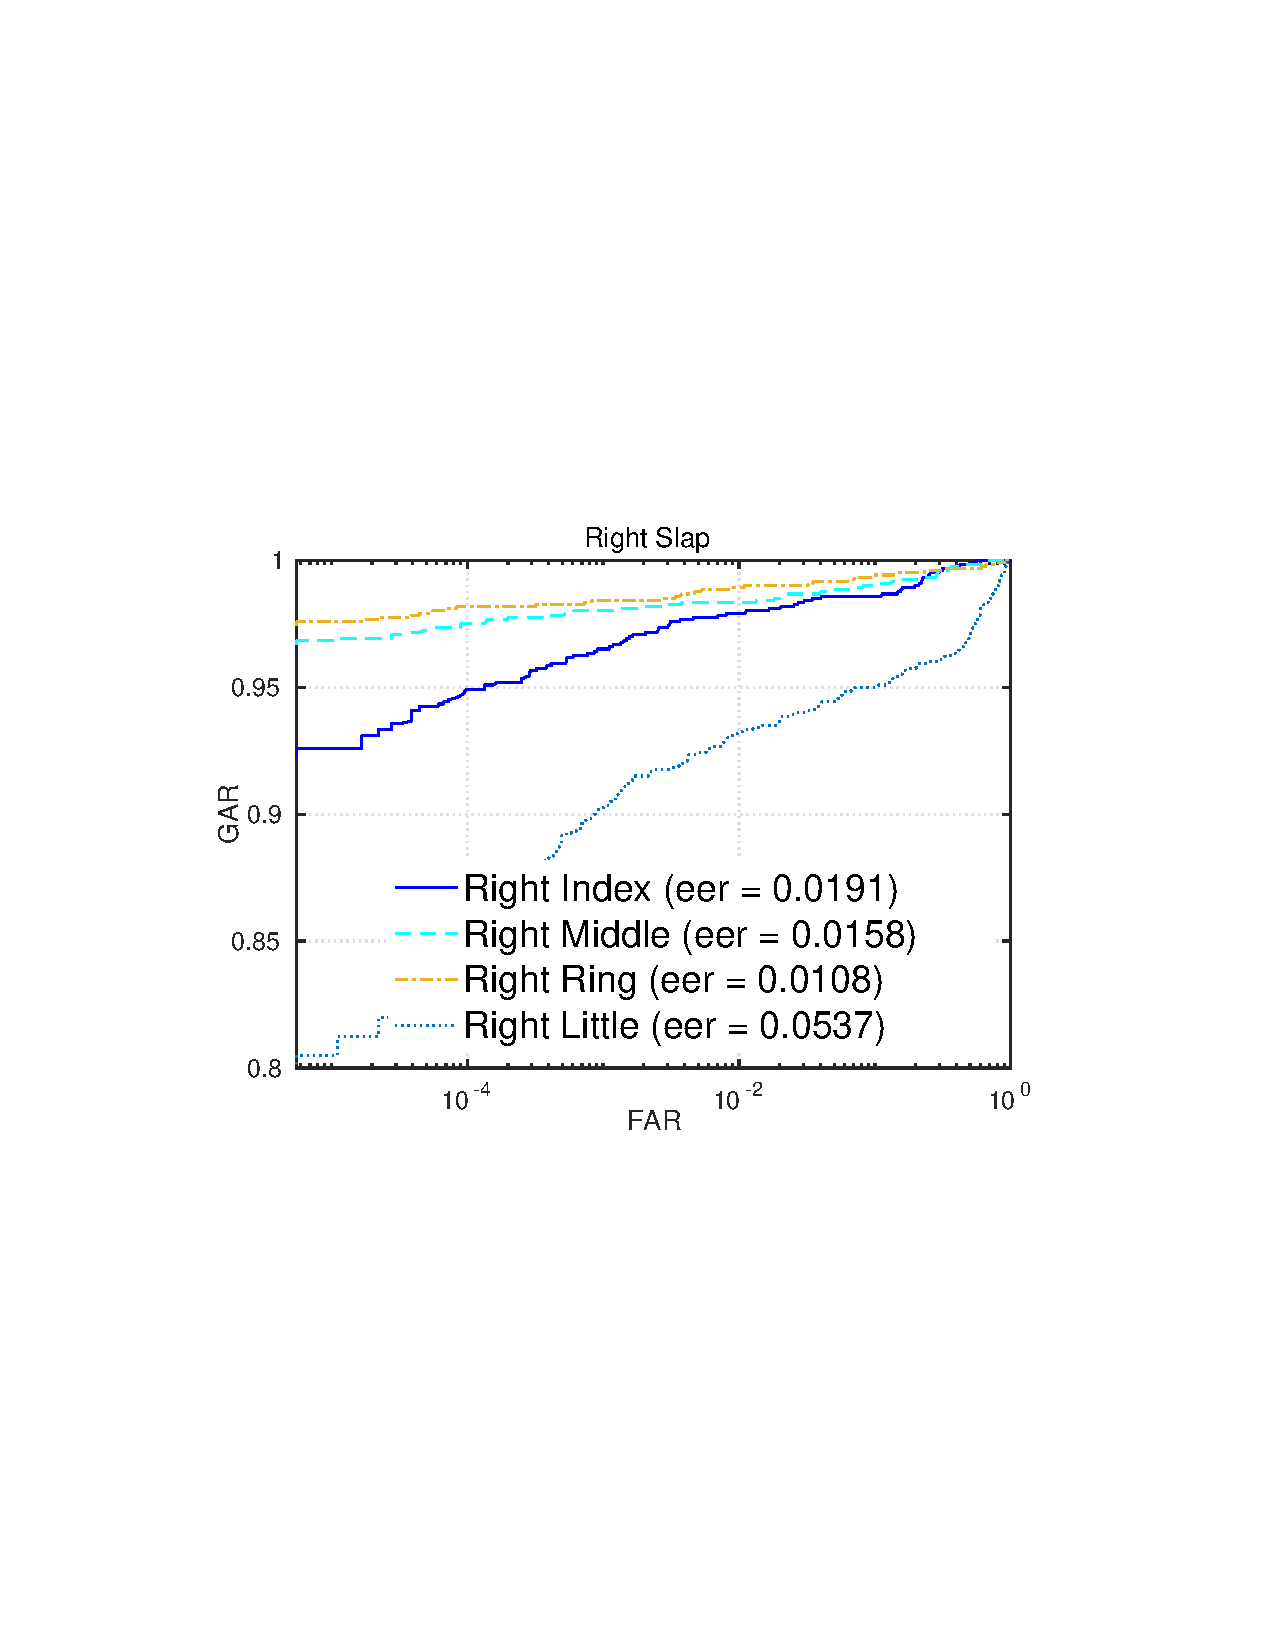
\includegraphics[width=1.75in]{Figures/finger-knuckle/right-roc.pdf}
    \label{}}

    \subfloat[]{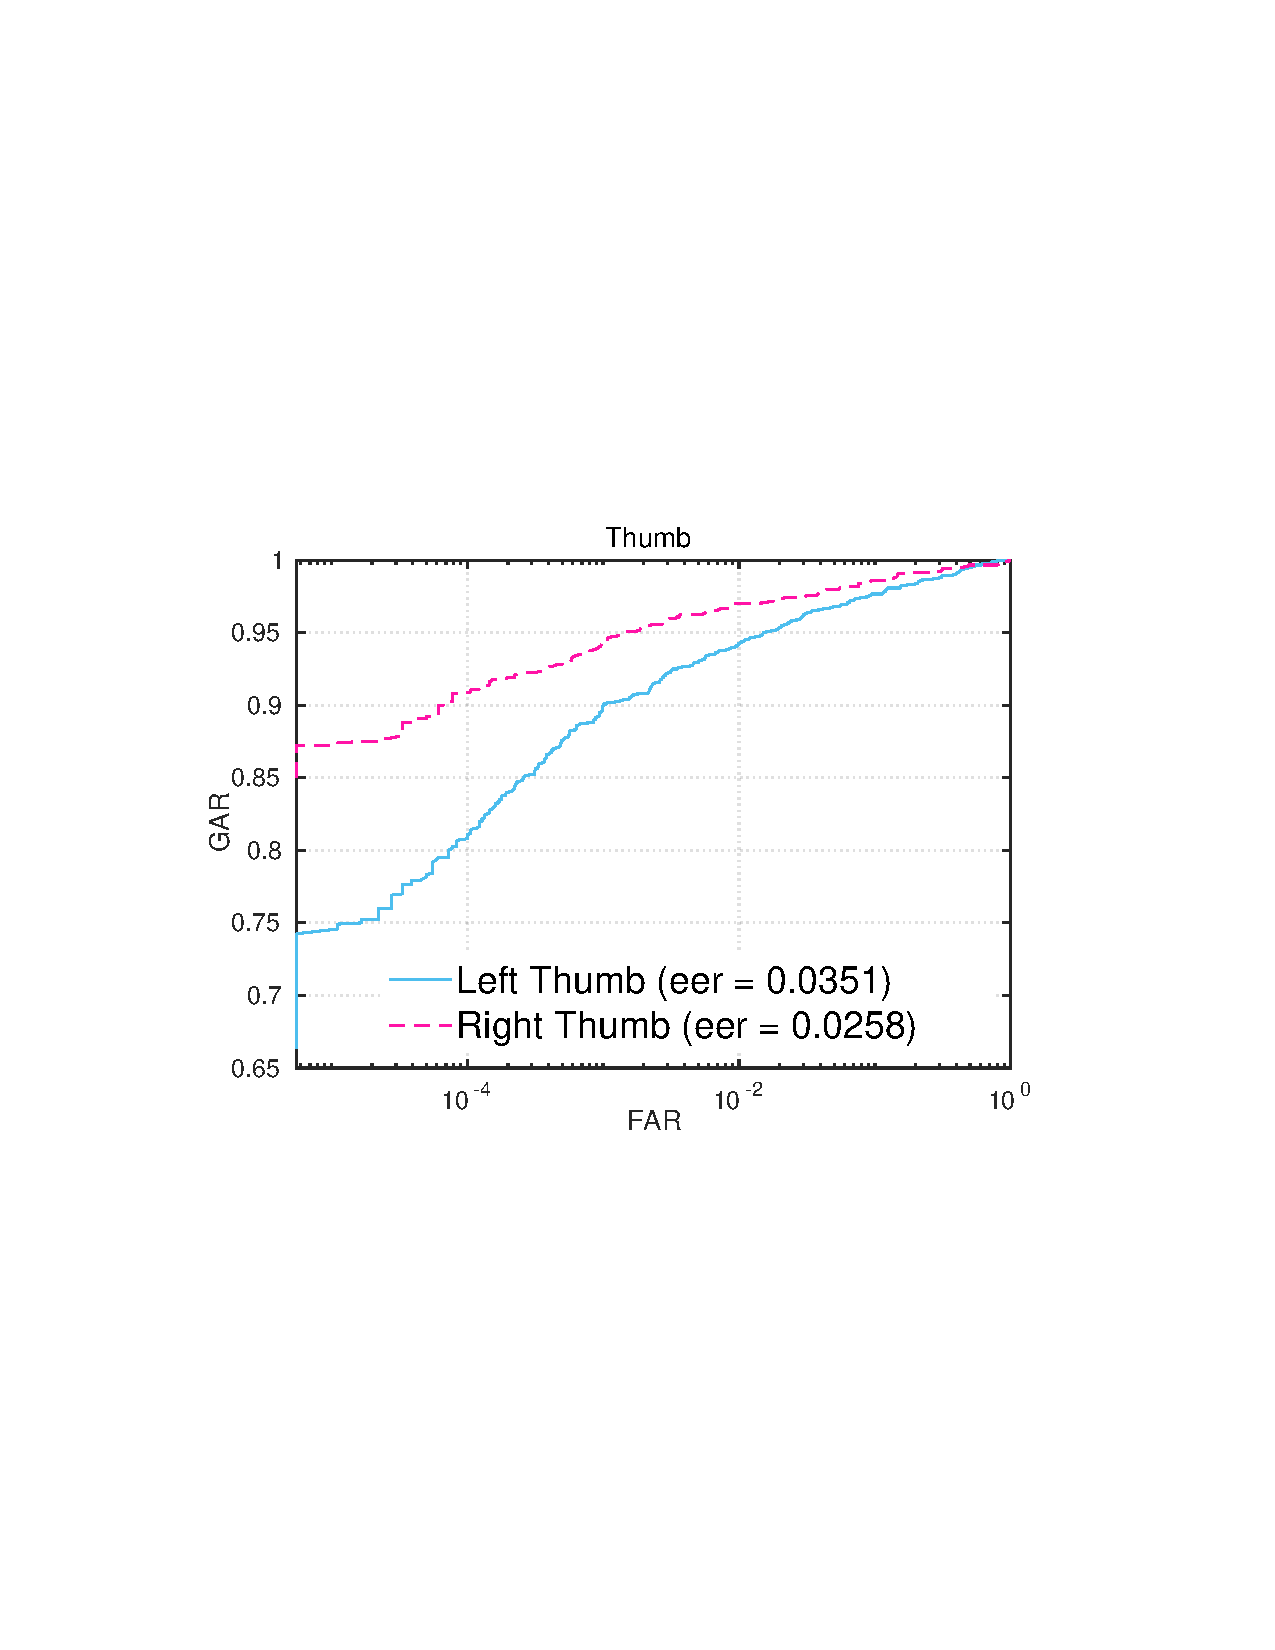
\includegraphics[width=1.8in]{Figures/finger-knuckle/thumb-roc.pdf}
    \label{}}
    \caption{Performance from the simultaneously acquired finger knuckle images from (a) left hand, (b) right hand, and (c) thumbs under 4-4-2 imaging protocols.}
    \label{fingerknuckle-performance}
\end{figure}

Each of the simultaneously acquired and segmented finger knuckle images were first evaluated for their individual performance. Fig. \ref{fingerknuckle-performance} illustrates receiver operating characteristics (ROC) for the finger knuckle images acquired from \textcolor{red}{each of nine different fingers (except the middle finger knuckle of left hand)}. These results indicate that the ring finger knuckle, from both the hands, offers superior performance followed by the performance from the middle finger, and then index finger. The performance from the knuckle from thumbs and the little finger is observed to be relatively poor. This can be largely attributed to the high agility \textcolor{red}{(which are easily deformed)} with the thumb and the little fingers which often results in degradation in the quality of segmented images. \textcolor{red}{This kind of conclusion also can be got from the Table \ref{summary-orientation}, the mean degree of ring finger knuckle of both hand is the lowest, while the mean degree of index and thumb finger knuckle are relatively large.} Fig. \ref{fingerknuckle-performance} also illustrates the equal error rate (EER) values for the respective finger knuckle images. \textcolor{red}{From the above figure, the lowest EER value is 0.0537 of little finger knuckle of right hand, which can show the generalized ability of our model. Because we only train our model on the middle finger knuckle of left hand.}

